\section{HellfireOS}
\label{sec:HellfireOS}
O HellfireOS \cite{hellfireos} é um sistema operacional de tempo real preemptivo que é parte constituinte
do Hellfire System (HFS). Projetado para sistemas MPSoC, possui gerenciamento
dinâmico de tarefas que conta com a proteção contra inversão de prioridades. Seu esclonador
possui as seguintes políticas de escalonamento:
Rate Monotonic, Round Robin, Earliest Deadline First e Deadline Monotonic.\\

Dentre as bibliotecas que nos interessam consta uma LibC customizada, uma math.h com emulação
de número de ponto flutuante e parte da pilha TCP.\\
A API do hellfire é dividida em 5 (cinco) grupos: Manipulação de Tarefas, Exclusão Mútua,
Manipulação de Memória, Comunicação entre Processos e LibC.\\
O Hellfire System conta também com uma plataforma para design que compreende diferentes
níveis de abstração, partindo de aplicações escritas em C, até a prototipação em FPGAs.
Isto é possível graças as ferramentas e módulos que fazem parte do Hellfire Framework (HFFW).
\subsection{Arquitetura}
\begin{figure}[H]
	\centering
		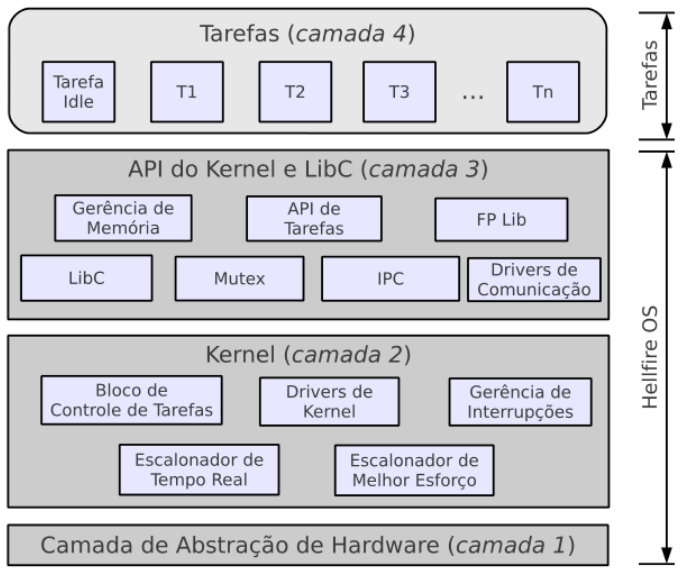
\includegraphics[width=\textwidth,height=\textheight,keepaspectratio]{fig/HellfireArch.png}
	\caption{Arquitetura em alto nível do HellfireOS.}
\end{figure}
%A API do HellfireOS é dividida em 5(cinco) grupos, a saber:
%\begin{itemize}
%	\item Manipulação de Tarefas
%	\item Exclusão Mútua
%	\item Manipulação de Memória
%	\item Comunicação entre processos
%	\item LibC
%\end{itemize}
